\section{Геометрия задачи}
1. Четырёхугольник $ABCD$ --- трапеция $(AD\parallel BC).$ Пусть $O$ --- точка пересечения диагоналей этой трапеции. Известно, что $\cfrac{S_{\Delta AOD}}{S_{\Delta BOC}}=16.$ Найти $\cfrac{BC}{AD}.$\\
2. Четырёхугольник $ABCD$ --- трапеция $(AD\parallel BC).$ Пусть $O$ --- точка пересечения диагоналей этой трапеции. Известно, что $\cfrac{S_{\Delta BOC}}{S_{\Delta AOD}}=\cfrac{1}{81}.$ Найти $\cfrac{AD}{BC}.$\\
3. В окружность радиуса $R$ вписан треугольник, одна сторона которого равна $R,$ а другая --- $R\sqrt{3}.$ Найти площадь этого треугольника.\\
4. В окружность радиуса $R$ вписан треугольник, одна сторона которого равна $\cfrac{3}{2}R,$ а другая --- $\cfrac{R\sqrt{7}}{2}.$ Найти площадь этого треугольника.\\
5. Точка $M,$ расположенная вне окружности, соединена с концами диаметра $AB.$ Прямая $MA$ пересекает окружность в точке $E,\ AE=3,\ ME=2,$ радиус окружности равен 2,5. Найдите площадь треугольника $AMB.$\\
6. Из точки $M,$ расположенной вне окружности, проведена касательная $MA$ к этой окружности ($A$ --- точка касания). Пусть $AC$ --- диаметр окружности, $MC$ пересекает окружность в точке $E,\ MA=5,$ радиус окружности равен 6. Найти $AE.$\\
7. В треугольнике $ABC: p(p-a)=\cfrac{3}{4}bc\ (a,\ b,\ c$ --- стороны, $p=\frac{a+b+c}{2}).$ Найти угол треугольника при вершине $A.$\\
8. В треугольнике $ABC: S=\cfrac{1}{4}(b^2+c^2-a^2)\ (a,\ b,\ c$ --- стороны, $S$ --- площадь). Найти угол треугольника при вершине $A.$\\
9. В треугольнике $ABC$ на стороне $AC$ взята точка $K$ так, что $AK=KC=3,$ а на стороне $BC$ взята точка $L$ так, что $BL=1,\ LC=2.$ Найти отношение площадей частей, на которые треугольник $ABC$ делится отрезком $KL.$\\
10. В треугольнике $ABC$ на стороне $AC$ взята точка $S$ так, что $AS=SC=6,$ а на стороне $AB$ взята точка $T$ так, что $AT=2,\ TB=4.$ Найти отношение площадей частей, на которые треугольник $ABC$ делится отрезком $ST.$\\
11. В окружности с центром $O$ проведена хорда $AB,$ пересекающая диаметр $CD$ в точке $K.$ Расстояние от  $O$ до $AB$ равно 4, $AB=16.$ Найти $OC.$\\
12. В окружности с центром $O$ проведена хорда $AB,$ пересекающая диаметр $CD$ в точке $K.$ Расстояние от  $O$ до $AB$ равно 4, $OC=10.$ Найти $AB.$\\
13. В равнобедренную трапецию с основаниями 2 и 8 вписана окружность. Другая окружность касается большего основания, боковой стороны и данной окружности. Найти радиус этой окружности.\\
14. В равнобедренную трапецию с боковой стороной 10 вписана окружность радиуса 4. Другая окружность касается большего основания, боковой стороны и данной окружности. Найти радиус этой окружности.\\
15. Основание $AC$ равнобедренного треугольника $ABC$ равно 6, а боковая сторона --- 5. Найти расстояние между точками пересечения медиан и высот треугольника $ABC.$\\
16. Основание $AC$ равнобедренного треугольника $ABC$ равно 6, а боковая сторона --- 5. Найти расстояние между точками пересечения медиан и биссектрис треугольника $ABC.$\\
17. Пусть $ABCD$ --- трапеция $(BC\parallel AD),\ S_{\Delta BOC}=a^2,\ S_{\Delta AOD}=b^2.$ Найти площадь трапеции.\\
18. По одну сторону от прямой $AC$ отложены отрезки $AB$ и $CD\ (AB\parallel CD),\ F$ --- точка пересечения $BC$ и $AD,\ FE\parallel AB,$ где $E$ --- точка на $AC.$ Доказать, что $\cfrac{1}{EF}=\cfrac{1}{AB}+\cfrac{1}{CD}.$\\
19. На катетах прямоугольного треугольника площади 1 как на диаметрах построены полукруги, расположенные вне этого треугольника. Найти сумму площадей этих полукругов, расположенных вне круга, описанного около исходного треугольника.\\
20. Даны две концентрические окружности. Проведена хорда большей окружности, касающаяся меньшей. На ней, как на диаметре, построена третья окружность. Доказать, что площадь третьего круга равна площади кольца между двумя первыми окружностями.\\
21. Найти площадь трапеции с основаниями 16 см и 44 см и боковыми сторонами 17 см и 25 см.\\
22. Найти площадь трапеции с основаниями 6 см и 7 см и боковыми сторонами 5 см и 12 см.\\
23. Основания трапеции 4 см и 16 см. Найти радиусы вписанной и описанной окружностей этой трапеции, если известно, что эти окружности существуют.\\
24. Основания трапеции 2 см и 14 см. Радиус вписанной окружности равен 4 см. Найти радиус описанной окружности этой трапеции, если известно, что эта окружность существует.\\
25. В треугольнике $ABC: AC=\sqrt{2},\ \angle A=75^\circ,\ \angle C=60^\circ.$ Найти $AB.$\\
26. В треугольнике $ABC: AB=\sqrt{3},\ \angle A=75^\circ,\ \angle B=45^\circ.$ Найти $AC.$\\
27. При каких $x$ векторы $\vec{a}=(4;5)$ и $\vec{b}=(x;-6)$ будут перпендикулярны?\\
28. При каких $x$ векторы $\vec{a}=(5;4)$ и $\vec{b}=(x;-3)$ будут перпендикулярны?\\
29. Найти диагональ и площадь ромба, если его стороны равны 10 см, а другая диагональ равна 12 см.\\
30. Найти диагональ и площадь ромба, если его стороны равны 5 см, а другая диагональ равна 6 см.\\
31. Касательная к окружности из некоторой точки равна 20 см, а наибольшая секущая, проведённая из той же точки, равна 50 см. Найдите радиус окружности.\\
32. Касательная к окружности из некоторой точки равна 12 см, а наибольшая секущая, проведённая из той же точки, равна 36 см. Найдите радиус окружности.\\
33. При каких значениях $t$ векторы $\vec{a}=(1;t)$ и $\vec{b}=(t+2;-t)$ имеют равные длины?\\
34. При каких значениях $t$ векторы $\vec{a}=(1;-t)$ и $\vec{b}=(2-t;t)$ имеют равные длины?\\
35. В равнобедренном треугольнике высота равна 20, а основание относится к стороне как $4:3.$ Найдите радиус вписанного круга.\\
36. В равнобедренном треугольнике высота равна 10, а основание относится к стороне как $3:4.$ Найдите радиус вписанного круга.\\
37. Диагонали ромба равны 14 и 48 см. Найдите высоту ромба.\\
38. Диагонали ромба равны 24 и 10 см. Найдите высоту ромба.\\
39. Сумма внешних углов многоугольника равна сумме его внутренних углов. Найдите число сторон этого многоугольника.\\
40. Сумма внешних углов многоугольника в 3 раза меньше суммы его внутренних углов. Найдите число сторон этого многоугольника.\\
41. Диагональ равнобедренной трапеции является биссектрисой её острого угла и делит среднюю линию трапеции на отрезки длиной 7,5 см и 12,5 см. Вычислите длины сторон трапеции.\\
42. Около окружности описана равнобедренная трапеция, периметр которой равен 18 см. Вычислите длину её средней линии.\\
43. Вычислите радиус окружности, описанной около равнобедренного треугольника, боковая сторона которого равна 20 см, а угол при вершине $40^\circ.$\\
44. Вычислите радиус окружности, описанной около равнобедренного треугольника с основанием 10 см и углом при основании $30^\circ.$\\
45. В равнобедренном треугольнике $\cos$ угла при вершине равен $\cfrac{7}{9}.$ Найти $\sin$ и $\cos$ угла при основании.\\
46. В равнобедренном треугольнике $\cos$ угла при вершине равен $\cfrac{5}{9}.$ Найти $\sin$ и $\cos$ угла при основании.\\
47. В равнобедренном треугольнике центр вписанного круга делит высоту в отношении $12:5,$ а боковая сторона равна 60 см. Определить основание.\\
48. В равнобедренном треугольнике радиус вписанного круга составляет $\cfrac{2}{7}$ высоты, а периметр этого треугольника равен 56 см. Определите его стороны.\\
49. Дан $\Delta ABC.$ Угол $B$ равен $90^\circ,$ точка $M$ лежит на стороне $AC.$ Угол  $MBC$ равен $30^\circ,$\\ $|MC|=2\text{ см},\ |AB|=2\text{ см}.$ Найдите $|BC|.$\\
50. Дан $\Delta ABC.$ Угол $B$ равен $90^\circ,$ точка $M$ лежит на стороне $AC.$ Угол  $MBC$ равен $30^\circ,$\\ $|MC|=3\text{ см},\ |AB|=3\text{ см}.$ Найдите $|BC|.$\\
51. В окружность радиуса $\sqrt{12}$ вписан квадрат. На диагонали квадрата, как на основании, построен равносторонний треугольник, вокруг которого описана окружность. Найти радиус этой окружности.\\
52. В окружность, диаметр которой равен $\sqrt{12},$ вписан равносторонний треугольник. На его высоте, как на основании, построен правильный треугольник, в который вписана окружность. Найти радиус этой окружности.\\
53. В треугольнике $ABC$ проведена медиана $BM.$ На стороне $BC$ взята точка $N$ так, что\\ $CN=2BN.$ В каком отношении $AN$ и $BM$ делят друг друга?\\
54. В трапеции $ABCD\ (AD\parallel BC)\ AD=2BC.$ На стороне $CD$ взята точка $M$ так, что $DM=2CM.$ В каком отношении отрезок $AM$ и диагональ $BD$ делят друг друга?\\
55. Существует ли треугольник, две высоты которого больше 1м, а площадь меньше $1\text{см}^2?$ Не забудьте обосновать ответ.\\
56. Существует ли треугольник, все стороны которого больше 1м, а площадь меньше $1\text{см}^2?$ Не забудьте обосновать ответ.\\
57. Даны два утверждения:\\
а) Если все стороны вписанного многоугольника равны, то и все его углы равны.\\
б) Если все углы вписанного многоугольника равны, то и все его стороны равны.\\
Какое из этих утверждений верно, а какое нет? (Подсказка: рассмотрите четырёхугольники и пятиугольники).\\
58. Даны два утверждения:\\
а) Если все стороны описанного многоугольника равны, то и все его углы равны.\\
б) Если все углы описанного многоугольника равны, то и все его стороны равны.\\
Какое из этих утверждений верно, а какое нет? (Подсказка: рассмотрите четырёхугольники и пятиугольники).\\
59. Найти радиусы вписанной и описанной окружности для равнобедренного треугольника, у которого боковая сторона равна 13, а высота, проведённая к основанию, равна 5.\\
60. Радиус окружности, описанной вокруг тупоугольного равнобедренного треугольника $ABC$ с основанием $AC$ равен 2. Центр $O$ окружности удалён от $AC$ на 1. Найти площадь треугольника $ABC$ и радиус окружности, вписанной в треугольник.\\
61. Диагонали трапеции перпендикулярны. Высота трапеции равна 4, одна из диагоналей равна 5. Найти площадь трапеции.\\
62. Диагонали трапеции перпендикулярны. Средняя линия трапеции равна 6,5, а одна из диагоналей равна 5. Найти площадь трапеции.\\
63. Прямая, параллельная стороне $AC$ треугольника $ABC,$ пересекает стороны $AB$ и $BC$ в точках $K$ и $M$ соответственно. Найдите $KM,$ если $BK:KA=2:5,\ AC=21$см.\\
64. Прямая, параллельная стороне $AC$ треугольника $ABC,$ пересекает стороны $AB$ и $BC$ в точках $K$ и $M$ соответственно. Найдите $AC,$ если $BK:KA=3:4,\ KM=18$см.\\
65. Найдите длину медианы $BM$ треугольника $ABC,$ если известны координаты вершин треугольника: $A(2;5),\ B(0;0),\ C(4;3).$\\
66. Найдите длину медианы $BM$ треугольника $ABC,$ если известны координаты вершин треугольника: $A(-3;-2),\ B(-6;2),\ C(0;0).$\\
67. Биссектрисы углов $A$ и $B$ при боковой стороне $AB$ трапеции $ABCD$ пересекаются в точке $F.$ Найдите $AB,$ если $AF=24$см, $BF=10$см.\\
68. Биссектрисы углов $A$ и $B$ при боковой стороне $AB$ трапеции $ABCD$ пересекаются в точке $F.$ Найдите $AB,$ если $AF=24$см, $BF=18$см.\\
69. Радиус окружности, описанной около равнобедренного треугольника, равен 5 см, а высота, проведённая к основанию, равна 8 см. Найдите площадь треугольника.\\
70. Радиус окружности, описанной около равнобедренного треугольника, равен 10 см, а основание треугольника равно 12 см. Найдите площадь треугольника.\\
71. $ABC$ --- прямоугольный треугольник с прямым углом при вершине $A,\ AD$ --- высота треугольника, $AM$ --- биссектриса. Найдите $AD,$ если $MB=3,\ MC=1.$\\
72. $ABC$ --- прямоугольный треугольник с прямым углом при вершине $A,\ AD$ --- высота треугольника, $AM$ --- биссектриса. Найдите $AD,$ если $MB=2,\ MC=4.$\\
73. Найдите сумму квадратов сторон равнобедренного треугольника с углом при вершине $\alpha=\cfrac{\pi}{4}$ и стороной основания $a=1.$\\
74. Найдите сумму квадратов сторон равнобедренного треугольника с углом при вершине $\alpha=\cfrac{\pi}{6}$ и стороной основания $a=1.$\\
75. Найдите радиус окружности, описанной около трапеции, последовательные стороны которой равны 2 см, 1 см, 1 см, 1 см.\\
76. В треугольнике $ABC: \cos C=\cfrac{\sqrt{2}}{2},\ AC=BC=2\sqrt{2}.$ Найдите высоту $AH$ этого треугольника.\\
77. В равнобедренном треугольнике $ABC$ с основанием $AC$ сторона $AB$ равна 8, а $\cos A=\cfrac{\sqrt{7}}{4}.$ Найдите высоту треугольника $ABC,$ проведённую к основанию.\\
78. Найдите длину медианы $BM$ треугольника $ABC,$ если известны координаты вершин треугольника: $A(1;4),\ B(0;0),\ C(4;1).$\\
79. Найдите длину медианы $BM$ треугольника $ABC,$ если известны координаты вершин треугольника: $A(3;2),\ B(2;3),\ C(0;0).$\\
80. Острый угол прямоугольного треугольника равен $24^\circ.$ Найдите угол между высотой и медианой, проведёнными из вершины прямого угла.\\
81. Острый угол прямоугольного треугольника равен $53^\circ.$ Найдите угол между высотой и медианой, проведёнными из вершины прямого угла.\\
82. В параллелограмме $ABCD$ высота, опущенная на сторону $AB,$ равна $20,\ AD=25.$ Найдите синус угла $B.$\\
83. В параллелограмме $ABCD$ высота, опущенная на сторону $AB,$ равна $14,\ AD=28.$ Найдите синус угла $B.$\\
84. $ABCD$ --- выпуклый четырёхугольник, $O$ --- точка пересечения его диагоналей, $OB=OD,$\\$AO<OC.$ Докажите, что $\angle BAD>\angle BCD.$\\
85. В трапеции $ABCD\ (AD\parallel BC)\ \angle A=60^\circ,\ \angle D=30^\circ,\ AD=a,\ BC=b.$ Найдите:\\
а) площадь трапеции $ABCD,$\\
б) длину отрезка, соединяющего середины $BC$ и $AD.$\\
86. Около трапеции описана окружность. Периметр трапеции равен 22, средняя линия равна 5. Найдите боковую сторону трапеции.\\
87. Боковая сторона равнобедренной трапеции равна её меньшему основанию, угол при основании равен $60^\circ,$ большее основание равно 12. Найдите радиус описанной окружности этой трапеции.\\
88. Угол при вершине, противолежащей основанию равнобедренного треугольника, равен $30^\circ.$ Боковая сторона треугольника равна 10. Найдите площадь этого треугольника.\\
89. Угол при вершине, противолежащей основанию равнобедренного треугольника, равен $150^\circ.$ Боковая сторона треугольника равна 20. Найдите площадь этого треугольника.\\
90. Найдите абсциссу центра окружности, описанной около треугольника, вершины которого имеют координаты $(8;0),\ (0;6),\ (8;6).$\\
91. Найдите ординату центра окружности, описанной около треугольника, вершины которого имеют координаты $(8;0),\ (0;6),\ (8;6).$\\
92. Найдите площадь треугольника, медианы которого равны равны 3, 4 и 5.\\
93. Найдите площадь треугольника, медианы которого равны равны 12, 15 и 21.\\
94. Две окружности радиуса $r$ касаются друг друга. Кроме того, каждая из них касается извне третьей окружности радиуса $R$ в точках $A$ и $B$ соответственно. Найдите  $r,$ если $AB=12,\ R=8.$\\
95. Две окружности радиуса $r$ касаются друг друга. Кроме того, каждая из них касается изнутри третьей окружности радиуса $R$ в точках $A$ и $B$ соответственно. Найдите радиус $R,$ если $AB=11,\ r=5.$\\
96. В равнобедренном треугольнике $ABC$ угол при вершине $B$ равен $120^\circ,\ AC=2\sqrt{2}.$ Найдите длину медианы $AM.$\\
97. В параллелограмме $ABCD$ дано: $AD=2,$ угол $BAD$ равен $60^\circ,\ BE\perp AD,\ BE=2\sqrt{3}.$ Найдите длину большей диагонали параллелограмма.\\
98. В прямоугольную трапецию вписана окружность радиуса $R.$ Найдите стороны трапеции, если её меньшее основание равно $\cfrac{4}{3}R.$\\
99. Окружность вписана в равнобедренную трапецию с основаниями  $a$ и $b.$ Найдите диагональ трапеции.\\
100. Высота, опущенная на гипотенузу прямоугольного треугольника, делит его на треугольники, площади которых равны $6\text{см}^2$ и $54\text{см}^2.$ Найдите гипотенузу треугольника.\\
101. В треугольнике $ABC$ известно, что $AB:AC=3:5,\ AD$ --- биссектриса угла. Площадь треугольника $ABD$ равна $9\text{см}^2.$ Найдите площадь треугольника $ACD.$\\
102. Гипотенуза $BC$ прямоугольного треугольника $ABC$ равна 25 см. Найдите длину биссектрисы треугольника, проведённой из вершины $C,$ если $AC=7$см.\\
103. Гипотенуза $BC$ прямоугольного треугольника $ABC$ равна 24 см. Найдите длину биссектрисы треугольника, проведённой из вершины $B,$ если $AB=3$см.\\
104. Точки $A(1;2),\ B(5;3)$ и $D(1;18)$ являются тремя вершинами трапеции
$ABCD$ с основаниями $AD$ и $BC.$ Известно, что около трапеции можно описать окружность. Найдите площадь трапеции.\\
105. Точки $A(3;2),\ B(4;7)$ и $C(16;7)$ являются тремя вершинами трапеции
$ABCD$ с основаниями $AD$ и $BC.$ Известно, что около трапеции можно описать окружность. Найдите площадь трапеции.\\
106. В прямоугольную трапецию вписана окружность радиуса $R.$ Найдите стороны трапеции, если её большее основание равно $4R.$\\
107. В треугольнике $ABC$ на стороне $BC$ взяли точку $M$ так, что $BM:MC=5:4.$ Вычислите длину отрезка $AM,$ если $AB=12,\ AC=15,\ BC=18.$\\
108. В треугольнике $ABC$ на стороне $BC$ взяли точку $M$ так, что $BM:MC=4:5.$ Вычислите длину отрезка $AM,$ если $AB=12,\ AC=15,\ BC=18.$\\
109. В равнобедренном треугольнике $ABC\ (AB=BC)\ AB=25,\ AC=14.$\\
а) Найдите высоту треугольника, проведённую из вершины $C.$\\
б) Найдите радиус вписанной окружности треугольника $ABC.$\\
в) Найдите радиус описанной окружности треугольника $ABC.$\\
г) В треугольник вписан прямоугольник $KLMN\ (KL=2LM)$ так, что точки $K$ и $L$ лежат на стороне $AC,$ а точки $M$ и $N$ --- на сторонах $BC$ и $AB$ соответственно. Найдите длину $KL.$\\
110. В равнобедренном треугольнике $ABC$ выполнено $AB=BC=13,\ AC=10.$\\
а) Найдите высоту треугольника, проведённую из вершины $C.$\\
б) Найдите радиус вписанной окружности треугольника $ABC.$\\
в) Найдите радиус описанной окружности треугольника $ABC.$\\
г) В треугольник вписан прямоугольник $KLMN\ (LM=2KL)$ так, что точки $K$ и $L$ лежат на стороне $AC,$ а точки $M$ и $N$ --- на сторонах $BC$ и $AB$ соответственно. Найдите длину $KL.$\\
111. В трапеции $ABCD$ стороны оснований $AD=10,\ BC=4.$ Боковые стороны $AB=4,\ CD=6.$ Найдите высоту трапеции.\\
112. В трапеции $ABCD$ стороны оснований $AD=9,\ BC=5.$ Боковые стороны $AB=4,\ CD=5.$ Найдите высоту трапеции.\\
113. В равнобедренную трапецию вписана окружность. Найдите радиус этой окружности, если основания трапеции равны 4 и 9.\\
114. В равнобедренную трапецию вписана окружность. Найдите радиус этой окружности, если основания трапеции равны 49 и 16.\\
115. Катеты прямоугольного треугольника равны 15 см и 20 см. Найдите высоту, проведённую к гипотенузе и радиус вписанной в треугольник окружности.\\
116. Катет и гипотенуза прямоугольного треугольника равны 30 см и 50 см. Найдите высоту, проведённую к гипотенузе и радиус вписанной в треугольник окружности.\\
117. В треугольнике $ABC\ AB=3$ см, $BC=5$ см, $AC=\sqrt{14}$ см. Найдите а) длину медианы $CM$ б) площадь треугольника $ABC.$\\
118. В треугольнике $ABC\ AB=4$ см, $BC=\sqrt{13}$ см, $AC=3$ см. Найдите а) длину медианы $CM$ б) площадь треугольника $ABC.$\\
119. Найдите площадь трапеции, диагонали которой равны 3 см и 4 см, а средняя линия равна 2,5 см.\\
120. Найдите площадь трапеции, диагонали которой равны 6 см и 8 см, а средняя линия равна 5 см.\\
121. В треугольнике $ABC$ биссектриса угла $A$ делит высоту, проведённую из вершины $B,$ в отношении $5:4,$ считая от точки $B.$ Найдите радиус окружности, описанной около треугольника $ABC,$ если $BC=12$ см.\\
122. Радиус окружности, описанной около треугольника $ABC,$ равен 13 см, $BC=24$ см. Найдите, в каком отношении, считая от вершины $B,$ биссектриса угла $A$ делит высоту, проведённую из этой вершины.\\
123. Медианы треугольника $ABC,$ проведённые из вершин $B$ и $C,$ пересекаются под прямым углом. Найдите длину медианы треугольника, проведённой из вершины $A,$ если $BC=42$ см.\\
124. Медианы треугольника $ABC,$ проведённые из вершин $B$ и $C,$ пересекаются под прямым углом. Найдите $BC,$ если длина медианы треугольника, проведённой из вершины $A,$ равна 36 см.\\
125. В равнобедренную трапецию можно вписать окружность. Найдите площадь этой трапеции, если её основания равны 1 и 25.\\
126. Точка $M$ является серединой боковой стороны $AB$ трапеции $ABCD.$ Найдите площадь трапеции, если площадь треугольника $MCD$ равна $28\text{ см}^2.$\\
127. Точка $M$ является серединой боковой стороны $AB$ трапеции $ABCD.$ Найдите площадь треугольника $MCD,$ если площадь  трапеции равна $26\text{ см}^2.$\\
128. Найдите косинус угла $D$ выпуклого четырёхугольника $ABCD,$ если косинус угла $B$ равен $\cfrac{5}{6},\ AB=6,\ BC=4,\ CD=5,\ AD=8.$\\
129. Найдите косинус угла $C$ выпуклого четырёхугольника $ABCD,$ если косинус угла $A$ равен $-\cfrac{2}{3},\ AB=2,\ BC=3,\ CD=7,\ AD=6.$\\
130. Окружность, вписанная в треугольник $ABC,$ касается его сторон в точках $M, K$ и $P.$ Найдите углы треугольника $ABC,$ если углы треугольника $MKP$ равны $56^\circ,\ 57^\circ,\ 67^\circ.$\\
131. Окружность, вписанная в треугольник $ABC,$ касается его сторон в точках $M, K$ и $P.$ Найдите углы треугольника $ABC,$ если углы треугольника $MKP$ равны $46^\circ,\ 58^\circ,\ 76^\circ.$\\
132. В выпуклом четырёхугольнике $ABCD$ углы $ABD$ и $ACD$ равны. Найдите величину угла при вершине $A$ четырёхугольника, если углы $DBC$ и $CDB$ равны соответственно $53^\circ$ и $64^\circ.$\\
133. В выпуклом четырёхугольнике $ABCD$ углы $DBC$ и $DAC$ равны. Найдите величину угла при вершине $D$ четырёхугольника, если углы $BAC$ и $BCA$ равны соответственно $42^\circ$ и $37^\circ.$\\
134. В треугольнике $ABC: \angle A=24^\circ,\ \angle B=80^\circ.$ Найдите угол между прямой, содержащей высоту треугольника, проведённой из вершины $B$ и прямой, содержащей биссектрису внешнего угла при вершине $C.$\\
135. В треугольнике $ABC: \angle A=26^\circ,\ \angle B=70^\circ.$ Найдите угол между прямой, содержащей высоту треугольника, проведённой из вершины $B$ и прямой, содержащей биссектрису внешнего угла при вершине $C.$\\
136. В трапеции $ABCD$ основания $AD$ и $BC$ равны соответственно 44 и 16. Боковая сторона $AB$ равна 17, а $CD$ равна 25. Найдите площадь трапеции.\\
137. В трапеции $ABCD$ основания $AD$ и $BC$ равны соответственно 41 и 13. Боковая сторона $AB$ равна 17, а $CD$ равна 25. Найдите площадь трапеции.\\
138. В треугольнике $ABC$ стороны $AB=6,\ BC=3,\ AC=5.$ на стороне $AC$ взята точка $M$ так, что $\cfrac{AM}{MC}=\cfrac{3}{2}.$ Найдите отрезок $BM.$\\
139. В треугольнике $ABC$ стороны $AB=6,\ BC=3,\ AC=5.$ на стороне $AB$ взята точка $M$ так, что $\cfrac{AM}{MB}=\cfrac{1}{5}.$ Найдите отрезок $CM.$\\
140. В прямоугольном треугольнике точка касания вписанной окружности делит гипотенузу на отрезки 5 и 12. Найдите катеты треугольника.\\
141. В прямоугольном треугольнике точка касания вписанной окружности делит гипотенузу на отрезки 3 и 10. Найдите катеты треугольника.\\
142. В треугольнике $ABC: \cos \angle C=\cfrac{\sqrt{2}}{3},\ AC=BC=3\sqrt{7}.$ Найдите высоту $AH$ этого треугольника.\\
143. В треугольнике $ABC: \cos \angle C=\cfrac{\sqrt{7}}{4},\ AC=BC=8.$ Найдите высоту $BH$ этого треугольника.\\
144. По стене крепости, имеющей форму равностороннего треугольника со стороной 400 м, ходят часовые, которые вооружены луками с дальностью стрельбы 100 м. Какова площадь <<простреливаемой>> территории\\
а) снаружи крепости,\\
б) внутри крепости?\\
145. В $\Delta ABC$ проведены медианы $AM$ и $CN.$
$O$ --- их точка пересечения. Какую часть площади $\Delta ABC$ составляет площадь четырёхугольника $NBMO?$\\
146. В $\Delta ABC$ проведена медиана $BN$ и средняя линия $KM.$ $O$ --- их точка пересечения. Какую часть площади $\Delta ABC$ составляет площадь $\Delta OMN?$\\
147. $ABCD$ --- выпуклый четырёхугольник с прямыми углами $B$ и $D,\angle A=45^\circ, BC=4, CD=3\sqrt{2}.$ Найти $AC.$\\
148.$MKNP$ --- выпуклый четырёхугольник с прямыми углами $M, N; \angle P=120^\circ, KM=4, KN=6.$ Найти $PK.$\\
149. Прямая делит равнобедренный прямоугольный треугольник с гипотенузой $\sqrt{8}$ на две части. Найдите наибольшее произведение площадей этих частей.\\
150. Прямая делит ромб с диагоналями 2 и 4 на две части. Найдите наибольшее произведение площадей
этих частей.\\
151. $ABCD$ --- прямоугольник. Из вершин $B$ и $D$ на диагональ $AC$ опущены перпендикуляры $BM$ и $DN,$
причём $MN=15,$ а $BM=DN=4.$ Найдите площадь прямоугольника $ABCD.$\\
152. $ABCD$ --- прямоугольник. Из вершин $B$ и $D$ на диагональ $AC$ опущены перпендикуляры $BK$ и $DM,$ причём $BK=DM=6,$ а $KM=5.$ Найдите площадь прямоугольника $ABCD.$\\
153. На катетах прямоугольного треугольника площадью 12 как на диаметрах построены полукруги, расположенные вне этого треугольника. Найдите суммарную площадь частей этих полукругов, расположенных вне круга, описанного около этого треугольника.
\begin{figure}[h]
\center{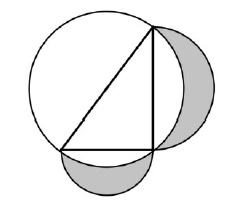
\includegraphics[scale=0.35]{rr.png}}
\end{figure}\\
154. Даны два полукруга, с диаметрами на одной прямой.
Хорда большего полукруга $AB$ длиной 12 параллельна диаметру и касается
меньшего полукруга. Найдите площадь закрашенной фигуры.
\begin{figure}[h]
\center{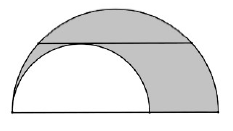
\includegraphics[scale=0.35]{rrr.png}}
\end{figure}\\
155. В трапеции $ABCD$ нижнее основание $AD$ в три раза больше верхнего. Точка $M$ лежит на боковой
стороне $CD,$ причём $CM:MD=1:3.$ Отрезок $AM$ пересекает диагональ $BD$ в точке $O.$ Найдите, в
каком отношении точка $O$ делит каждый из этих отрезков.\\
156. В треугольнике $ABC$ на стороне $BC$ взята точка $N,$ такая, что $BN : NC=3:2.$ Отрезок $AN$ и медиана
$BM$ пересекаются в точке $O.$ Найдите, в каком отношении точка $O$ делит каждый из этих отрезков.\\
157. Прямая, проведенная через середину $N$ стороны $AB$ квадрата $ABCD,$ пересекает сторону $AD$ в точке
$T,$ а продолжение стороны $CD$ в точке $M,$ и образует с прямой $AB$ угол, тангенс которого равен 0,5.
Сторона квадрата равна 8. Найдите площадь треугольника $BMT.$\\
158. Прямая, проведенная через середину $N$ стороны $AB$ квадрата $ABCD,$ пересекает прямые $CD$ и
$AD$ в точках $M$ и $T$ соответственно (так, что $T$ лежит на продолжении $DA$ за точку $A),$ и
образует с прямой $AD$ угол, тангенс которого равен 2. Сторона квадрата равна 6. Найдите площадь треугольника $BMT.$\\
159. Внутри угла величиной $45^\circ$ расположена точка $N,$ удалённая на расстояния $2\sqrt{2}$ и 2 см от сторон угла.
Найдите расстояние от точки $N$ до вершины угла.\\
160. Внутри угла величиной $60^\circ$ расположена точка $M,$ удалённая на расстояния $\sqrt{7}$ и $2\sqrt{7}$ см от
сторон угла. Найдите расстояние от точки $M$ до вершины угла.\\
161. Сторона параллелограмма равна 12см, а расстояние от точки пересечения диагоналей до этой стороны равно 4см. Найдите площадь параллелограмма.\\
162. Сторона параллелограмма равна 14см, а расстояние от точки пересечения диагоналей до этой стороны равно 3см. Найдите площадь параллелограмма.\\
163. В равнобедренном треугольнике $ABC\ (AB=BC)\ AB=25,\ AC=14.$\\
а) Найдите высоту треугольника, проведённую из вершины $C.$\\
б) Найдите радиус вписанной окружности треугольника $ABC.$\\
в) Найдите радиус описанной окружности треугольника $ABC.$\\
г) В треугольник вписан прямоугольник $KLMN\ (LM=2KL)$ так, что точки $K$ и $L$ лежат на стороне $AC,$ а точки $M$ и $N$ --- на сторонах $BC$ и $AB$ соответственно. Найдите длину $KL.$\\
164. $AC$ --- основание равнобедренного треугольника $ABC.$ Точка $D$ лежит на стороне $AC.$ $AD=4,\ DC=3.$ Окружности, вписанные в треугольники $ABD$ и $DBC,$ касаются $BD$ в точках $M$ и $N$ соответственно. Найдите длину отрезка $MN.$\\
165. $PK$ --- основание равнобедренного треугольника $SPK.$ Точка $F$ лежит на стороне $PK.$ $PF=1,\ FK=3.$ Окружности, вписанные в треугольники $PSF$ и $FSK,$ касаются $SF$ в точках $E$ и $O$ соответственно. Найдите длину отрезка $OE.$\\
166. Найдите площадь прямоугольного треугольника, если биссектриса прямого угла делит гипотенузу на отрезки длины 3 и 4.\\
167. Найдите площадь прямоугольного треугольника, если биссектриса прямого угла делит гипотенузу на отрезки длины 15 и 20.\\
168. Дан $\Delta ABC$ с углами $\angle A=40^\circ,\ \angle B=120^\circ,\ \angle C=20^\circ.$ В нём проведены высоты $AA_1,\ BB_1,$\\$ CC_1,\ H$ --- точка их пересечения. Найти: а) $\angle ACH$ б) $\angle HA_1C_1$ в) $\angle A_1B_1B$\\
169. Дана трапеция $ABCD$ с основаниями 15 и 20 и боковыми сторонами 4 и 5. Две окружности касаются обоих оснований трапеции и, кроме того, одной из боковых сторон $AB$ и $CD$ соответственно. Найти расстояние между центрами окружностей.\\
170. Дан $\Delta ABC:\ AB=30,\ AC=40,\ AL$ --- биссектриса, $M$ --- середина $AL.$ Площадь $\Delta BML$ равна 60. Найти площадь $\Delta MLC.$\\
171. $ABCD$ --- параллелограмм площадью 22. $AK$ --- биссектриса острого угла $A,$ точка $K\in BC,\ AB=5,\ AD=6,\ AK\cap BD=O.$ Найти площадь $\Delta BOK.$\\
172. $ABCD$ --- трапеция с основаниями $BC$ и $AD$ площадью 20. $CK$ --- биссектриса угла $C,$ точка $K\in AD,\ BC=3,\ AD=7, CD=5,\ CK\cap BD=O.$ Найти площадь $\Delta BOC.$\\
173. $AC$ --- основание р/б $\Delta ABC,\ D\in AC,\ AD=4,\ CD=2.$ Окружности, вписанные в $\Delta ABD$ и $\Delta DBC,$ касаются $BD$ в точках $M$ и $N$ соответственно. Найти длину отрезка $MN.$\\
174. $PK$ --- основание р/б $\Delta SPK,\ F\in PK,\ FK=3.$ Окружности, вписанные в $\Delta PSF$ и $\Delta FSK,$ касаются $SF$ в точках $E$ и $O$ соответственно. Найти длину отрезка $OE.$\\
175. В треугольнике $ABC$ известны длины двух сторон $|AB|=6,\ |AC|=4.$ Биссектриса $CK$ делит медиану $AM$ пополам.\\
а) Найдите $|AK|.$\\
б) Найдите косинус наибольшего угла треугольника $ABC.$\\
в) Найдите $|AT|,$ где $T$ --- точка пересечения прямой $AM$ с описанной около $\Delta ABC$ окружностью.\\
176. В равнобедренном треугольнике $ABC$ с основанием $BC\ AB=17,\ BC=16.$ Найдите $a)$ высоту из точки $B,\ b)$ радиус вписанной окружности, $c)$ радиус описанной окружности.\\
177. В треугольнике $ABC\ AB=8,\ BC=12,\ AC=10.$ Найдите длину биссектрисы $BL.$\\
178. Сторона $AD$ вписанного четырёхугольника $ABCD$ является диаметром его описанной окружности, $M$ --- точка пересечения диагоналей, $H$ --- проекция точки $M$ на $AD.$ Докажите, что $M$ --- центр вписанной окружности треугольника $BHC.$\\
179. Точка $K$ на медиане $BM$ треугольника $ABC$ такова, что $BK:KM=3:1.$ В каком отношении прямая $CK$ делит отрезок $AB?$\\
180. Дан угол с вершиной в точке $O$ величиной $60^\circ.$ Внутри этого угла взята точка $A,$ равноудалённая от сторон угла. Известно, что $OA=8.$ Найдите длину окружности с центром в $A,$ касающейся сторон угла.\\
181. Дан угол с вершиной в точке $O$ величиной $120^\circ.$ В этот угол вписан круг площади $81\pi.$ Найдите расстояние от центра этого круга до точки $O.$\\
182. В треугольнике $ABC$ проведены медиана $BM$ и отрезок $AN,$ где точка $N$ лежит на стороне $BC,$ причём $BN:BC=0,4.$ Отрезки $BM$ и $AN$ пересекаются в точке $O.$ Найдите $BO:OM.$\\
183. В треугольнике $KLM$ проведены медиана $MA$ и отрезок $KB,$ где точка $B$ лежит на стороне $ML,$ причём $LB:BM=2:3.$ Отрезки $MA$ и $KB$ пересекаются в точке $O.$ Найдите $KO:KB.$\\
184. Площадь треугольника $ABC$ равна $5\sqrt{5},$ при этом $AB=3\sqrt{5},\ AC=2\sqrt{5}.$ Найдите периметр данного треугольника.\\
185. Площадь треугольника $ABC$ равна 32, при этом $AB=10,\ \cos(\angle A)=0,6.$ Найдите периметр данного треугольника.\\
186. В трапеции $ABCD$ с основаниями $AD$ и $BC$ известны длины всех сторон: $AB=5,\ BC=8,\ CD=4,\ AD=10.$ Найдите расстояние от точки $C$ до прямой $AB.$\\
187. В трапеции $ABCD$ даны длины оснований $AD=12$ и $BC=8,$ а также длины диагоналей $AC=10$ и $BD=18.$ Найдите расстояние от точки $D$ до прямой $AC.$\\
188. Дан треугольник $ABC,$ в котором $\angle B=90^\circ.$ Пусть $BK$ --- высота этого треугольника. Известно, что $BC=40,\ BK=24.$ Найдите расстояние между центрами окружностей, вписанных в треугольники $ABK$ и $BKC.$\\
189. Дан треугольник $ABC$ с прямым углом при вершине $B.$ Пусть $BK$ --- высота этого треугольника. Известно, что $AB=18,\ KC=19,2.$ В треугольник $BKC$ вписана окружность с центром $O.$ Найдите расстояние между точкой $O$ и центром окружности, описанной около треугольника $ABC.$\\
190. В ромбе со стороной 17 одна из диагоналей имеет длину 16. Найдите радиус вписанной в этот ромб окружности.\\
191. Из точки $X$ к окружности проведены касательная и секущая. Расстояние от $X$ до точки касания равно 9, а расстояние от $X$ до одной из точек пересечения окружности и секущей равно 27. Найдите радиус окружности, если расстояние от центра до секущей равно 5.\\
192. В треугольнике $ABC$ медиана $AM$ и биссектриса $BL$ перпендикулярны и пересекаются в точке $F.$ Найдите площадь треугольника $ABC,$ если площадь треугольника $FML$ равна 1.\\
193. Точки $M$ и $N$ --- середины сторон $AB$ и $BC$ треугольника $ABC$ соответственно, $BL$ --- его биссектриса. Оказалось, что четырёхугольник $MBNL$ вписан в окружность радиуса $8\sqrt{3},$ а $AL:LC=2:3.$ Найдите $MN.$\\
194. Основания равнобедренной трапеции равны 7 и 25, а боковые стороны --- 15. Докажите, что центр окружности, описанной около трапеции, лежит на её большем основании.\\
195. Биссектриса $AL$ треугольника $ABC$ перпендикулярна его медиане $BM.$ Найдите площадь этого треугольника, если известно, что $AB=\sqrt{3},\ ML=1.$\\
196. В четырёхугольник $ABCD$ вписана окружность. $E$ --- точка касания окружности со стороной $AB.$ Продолжения сторон $AB$ и $CD$ пересекаются в точке $P.$ Найдите длину отрезка $EP,$ если периметр $\Delta BKP$ равен 8.\\
197. В четырёхугольник $AKPC$ вписана окружность. $E$ --- точка касания окружности со стороной $AK.$ Продолжения сторон $AK$ и $PC$ пересекаются в точке $B.$ Найдите периметр $\Delta BKP,$ если $BE=7.$\\
198. Трапеция делится диагоналями на 4 треугольника с площадями $A,\ B,\ C$ и $D.$ $A=3,\ D=12.$ Найдите площадь трапеции.\\
199. Трапеция делится диагоналями на 4 треугольника с площадями $A,\ B,\ C$ и $D.$ $A=4,\ D=8.$ Найдите площадь трапеции.\\
200. Пусть $a,b,c$ --- длины сторон треугольника, $S$ --- его площадь. Докажите неравенство $6S<ab+bc+ac.$\\
201. Найдите все прямоугольные треугольники, длины сторон которых выражаются целыми числами, если известно, что гипотенуза на 1 больше одного из катетов, а косинус угла между этими сторонами меньше $\cfrac{29}{30}.$\\
202. В неравнобедренном прямоугольном треугольнике $ABC$ с прямым углом $B$ точка $C_1$ симметрична точке $C$ относительно прямой, содержащей медиану $BM.$ Найдите $\angle AC_1B,$ если $\angle BAC=\alpha.$\\
203. Площадь треугольника $ABC$ равна $S.$ Точка $M$ --- середина его стороны $BC,$ а точка $K$ делит сторону $AC$ в отношении $AK:KC=2:1.$ Отрезки $AM$ и $BK$ пересекаются в точке $O.$ Найдите площадь четырёхугольника $OMCK.$\\
204. На сторонах прямого угла с вершиной $M$ выбраны точки $D$ и $K$ так, что $MD : MK = 7.$ На
биссектрисе угла $DMK$ взята точка $E,$ равноудалённая от $D$ и $K.$ Найдите $DK,$ если $ME = 4.$\\
205. На сторонах прямого угла с вершиной $B$ выбраны точки $A$ и $C$ так, что $AB : CB = 4 : 3.$ На
биссектрисе $ABC$ взята точка $K,$ равноудалённая от $A$ и $C.$ Найдите $AC,$ если $BK =\cfrac{7\sqrt{2}}{2}.$\\
206. Боковые стороны трапеции равны 15 см и 20 см, а основания равны 6 см и 31 см. Найдите угол между прямыми, содержащими боковые стороны трапеции.\\
207. Диагонали трапеции равны 10 см и 24 см, а основания равны 7 см и 19 см. Найдите угол между прямыми, содержащими диагонали трапеции.\\
208. Круги радиусов 3, 7 и 10 касаются друг друга внешним образом. Найдите радиус окружности, вписанной в треугольник с вершинами в центрах этих кругов.\\
209. Круги радиусов 5, 6 и 9 касаются друг друга внешним образом. Найдите радиус окружности, вписанной в треугольник с вершинами в центрах этих кругов.\\
210. В $\Delta ABC:\; |AB| = 3,\ |BC| = 5,\ |CA| = 7, O$ --- центр вписанной в треугольник окружности.
Разложите вектор  $\overline{BO}$ по векторам  $\overline{AB}=\vec{b}$ и  $\overline{AC}=\vec{c}.$\\
211. В $\Delta ABC:\; |AB| = 3,\ |BC| = 5,\ |CA| = 7,\ O$ --- центр вписанной в треугольник окружности. Разложите вектор $\overline{CO}$ по векторам
$\overline{AB}=\vec{b}$ и  $\overline{AC}=\vec{c}.$\\
212. В трапеции  $ABCD$ длина основания  $AD$ равна  $2\sqrt{2},$ а длина основания  $BC$ равна  $\sqrt{2}.$ Угол $A=15^\circ,$
угол $D=30^\circ.$ Найдите длину боковой стороны  $AB.$\\
213. Высоты  $AK$ и  $CL$ остроугольного треугольника  $ABC$ пересекаются в точке  $H.$ Найдите тангенс угла
$BAC,$ если  $AH=HK$ и  $CH=2HL.$\\
214. В трапеции  $ABCD\  (AD\parallel BC)$ из точки  $E$ --- середины  $CD$ провели перпендикуляр  $EF$ к прямой  $AB.$
Найдите площадь трапеции, если  $AB=5,\ EF=4.$\\
215. На стороне  $AC$ треугольника  $ABC$ как на диаметре построена окружность радиуса 10 см. Эта
окружность пересекает стороны  $AB$ и  $BC$ в точках  $X$ и  $Y$ соответственно. Найдите  $AX\cdot AB + CY\cdot BC.$
\newpage
